\documentclass[11pt]{article}

    \usepackage[breakable]{tcolorbox}
    \usepackage{parskip} % Stop auto-indenting (to mimic markdown behaviour)
    
    \usepackage{iftex}
    \ifPDFTeX
    	\usepackage[T1]{fontenc}
    	\usepackage{mathpazo}
    \else
    	\usepackage{fontspec}
    \fi

    % Basic figure setup, for now with no caption control since it's done
    % automatically by Pandoc (which extracts ![](path) syntax from Markdown).
    \usepackage{graphicx}
    % Maintain compatibility with old templates. Remove in nbconvert 6.0
    \let\Oldincludegraphics\includegraphics
    % Ensure that by default, figures have no caption (until we provide a
    % proper Figure object with a Caption API and a way to capture that
    % in the conversion process - todo).
    \usepackage{caption}
    \DeclareCaptionFormat{nocaption}{}
    \captionsetup{format=nocaption,aboveskip=0pt,belowskip=0pt}

    \usepackage[Export]{adjustbox} % Used to constrain images to a maximum size
    \adjustboxset{max size={0.9\linewidth}{0.9\paperheight}}
    \usepackage{float}
    \floatplacement{figure}{H} % forces figures to be placed at the correct location
    \usepackage{xcolor} % Allow colors to be defined
    \usepackage{enumerate} % Needed for markdown enumerations to work
    \usepackage{geometry} % Used to adjust the document margins
    \usepackage{amsmath} % Equations
    \usepackage{amssymb} % Equations
    \usepackage{textcomp} % defines textquotesingle
    % Hack from http://tex.stackexchange.com/a/47451/13684:
    \AtBeginDocument{%
        \def\PYZsq{\textquotesingle}% Upright quotes in Pygmentized code
    }
    \usepackage{upquote} % Upright quotes for verbatim code
    \usepackage{eurosym} % defines \euro
    \usepackage[mathletters]{ucs} % Extended unicode (utf-8) support
    \usepackage{fancyvrb} % verbatim replacement that allows latex
    \usepackage{grffile} % extends the file name processing of package graphics 
                         % to support a larger range
    \makeatletter % fix for grffile with XeLaTeX
    \def\Gread@@xetex#1{%
      \IfFileExists{"\Gin@base".bb}%
      {\Gread@eps{\Gin@base.bb}}%
      {\Gread@@xetex@aux#1}%
    }
    \makeatother

    % The hyperref package gives us a pdf with properly built
    % internal navigation ('pdf bookmarks' for the table of contents,
    % internal cross-reference links, web links for URLs, etc.)
    \usepackage{hyperref}
    % The default LaTeX title has an obnoxious amount of whitespace. By default,
    % titling removes some of it. It also provides customization options.
    \usepackage{titling}
    \usepackage{longtable} % longtable support required by pandoc >1.10
    \usepackage{booktabs}  % table support for pandoc > 1.12.2
    \usepackage[inline]{enumitem} % IRkernel/repr support (it uses the enumerate* environment)
    \usepackage[normalem]{ulem} % ulem is needed to support strikethroughs (\sout)
                                % normalem makes italics be italics, not underlines
    \usepackage{mathrsfs}
    

    
    % Colors for the hyperref package
    \definecolor{urlcolor}{rgb}{0,.145,.698}
    \definecolor{linkcolor}{rgb}{.71,0.21,0.01}
    \definecolor{citecolor}{rgb}{.12,.54,.11}

    % ANSI colors
    \definecolor{ansi-black}{HTML}{3E424D}
    \definecolor{ansi-black-intense}{HTML}{282C36}
    \definecolor{ansi-red}{HTML}{E75C58}
    \definecolor{ansi-red-intense}{HTML}{B22B31}
    \definecolor{ansi-green}{HTML}{00A250}
    \definecolor{ansi-green-intense}{HTML}{007427}
    \definecolor{ansi-yellow}{HTML}{DDB62B}
    \definecolor{ansi-yellow-intense}{HTML}{B27D12}
    \definecolor{ansi-blue}{HTML}{208FFB}
    \definecolor{ansi-blue-intense}{HTML}{0065CA}
    \definecolor{ansi-magenta}{HTML}{D160C4}
    \definecolor{ansi-magenta-intense}{HTML}{A03196}
    \definecolor{ansi-cyan}{HTML}{60C6C8}
    \definecolor{ansi-cyan-intense}{HTML}{258F8F}
    \definecolor{ansi-white}{HTML}{C5C1B4}
    \definecolor{ansi-white-intense}{HTML}{A1A6B2}
    \definecolor{ansi-default-inverse-fg}{HTML}{FFFFFF}
    \definecolor{ansi-default-inverse-bg}{HTML}{000000}

    % commands and environments needed by pandoc snippets
    % extracted from the output of `pandoc -s`
    \providecommand{\tightlist}{%
      \setlength{\itemsep}{0pt}\setlength{\parskip}{0pt}}
    \DefineVerbatimEnvironment{Highlighting}{Verbatim}{commandchars=\\\{\}}
    % Add ',fontsize=\small' for more characters per line
    \newenvironment{Shaded}{}{}
    \newcommand{\KeywordTok}[1]{\textcolor[rgb]{0.00,0.44,0.13}{\textbf{{#1}}}}
    \newcommand{\DataTypeTok}[1]{\textcolor[rgb]{0.56,0.13,0.00}{{#1}}}
    \newcommand{\DecValTok}[1]{\textcolor[rgb]{0.25,0.63,0.44}{{#1}}}
    \newcommand{\BaseNTok}[1]{\textcolor[rgb]{0.25,0.63,0.44}{{#1}}}
    \newcommand{\FloatTok}[1]{\textcolor[rgb]{0.25,0.63,0.44}{{#1}}}
    \newcommand{\CharTok}[1]{\textcolor[rgb]{0.25,0.44,0.63}{{#1}}}
    \newcommand{\StringTok}[1]{\textcolor[rgb]{0.25,0.44,0.63}{{#1}}}
    \newcommand{\CommentTok}[1]{\textcolor[rgb]{0.38,0.63,0.69}{\textit{{#1}}}}
    \newcommand{\OtherTok}[1]{\textcolor[rgb]{0.00,0.44,0.13}{{#1}}}
    \newcommand{\AlertTok}[1]{\textcolor[rgb]{1.00,0.00,0.00}{\textbf{{#1}}}}
    \newcommand{\FunctionTok}[1]{\textcolor[rgb]{0.02,0.16,0.49}{{#1}}}
    \newcommand{\RegionMarkerTok}[1]{{#1}}
    \newcommand{\ErrorTok}[1]{\textcolor[rgb]{1.00,0.00,0.00}{\textbf{{#1}}}}
    \newcommand{\NormalTok}[1]{{#1}}
    
    % Additional commands for more recent versions of Pandoc
    \newcommand{\ConstantTok}[1]{\textcolor[rgb]{0.53,0.00,0.00}{{#1}}}
    \newcommand{\SpecialCharTok}[1]{\textcolor[rgb]{0.25,0.44,0.63}{{#1}}}
    \newcommand{\VerbatimStringTok}[1]{\textcolor[rgb]{0.25,0.44,0.63}{{#1}}}
    \newcommand{\SpecialStringTok}[1]{\textcolor[rgb]{0.73,0.40,0.53}{{#1}}}
    \newcommand{\ImportTok}[1]{{#1}}
    \newcommand{\DocumentationTok}[1]{\textcolor[rgb]{0.73,0.13,0.13}{\textit{{#1}}}}
    \newcommand{\AnnotationTok}[1]{\textcolor[rgb]{0.38,0.63,0.69}{\textbf{\textit{{#1}}}}}
    \newcommand{\CommentVarTok}[1]{\textcolor[rgb]{0.38,0.63,0.69}{\textbf{\textit{{#1}}}}}
    \newcommand{\VariableTok}[1]{\textcolor[rgb]{0.10,0.09,0.49}{{#1}}}
    \newcommand{\ControlFlowTok}[1]{\textcolor[rgb]{0.00,0.44,0.13}{\textbf{{#1}}}}
    \newcommand{\OperatorTok}[1]{\textcolor[rgb]{0.40,0.40,0.40}{{#1}}}
    \newcommand{\BuiltInTok}[1]{{#1}}
    \newcommand{\ExtensionTok}[1]{{#1}}
    \newcommand{\PreprocessorTok}[1]{\textcolor[rgb]{0.74,0.48,0.00}{{#1}}}
    \newcommand{\AttributeTok}[1]{\textcolor[rgb]{0.49,0.56,0.16}{{#1}}}
    \newcommand{\InformationTok}[1]{\textcolor[rgb]{0.38,0.63,0.69}{\textbf{\textit{{#1}}}}}
    \newcommand{\WarningTok}[1]{\textcolor[rgb]{0.38,0.63,0.69}{\textbf{\textit{{#1}}}}}
    
    
    % Define a nice break command that doesn't care if a line doesn't already
    % exist.
    \def\br{\hspace*{\fill} \\* }
    % Math Jax compatibility definitions
    \def\gt{>}
    \def\lt{<}
    \let\Oldtex\TeX
    \let\Oldlatex\LaTeX
    \renewcommand{\TeX}{\textrm{\Oldtex}}
    \renewcommand{\LaTeX}{\textrm{\Oldlatex}}
    % Document parameters
    % Document title
    \title{Chapter2}
    
    
    
    
    
% Pygments definitions
\makeatletter
\def\PY@reset{\let\PY@it=\relax \let\PY@bf=\relax%
    \let\PY@ul=\relax \let\PY@tc=\relax%
    \let\PY@bc=\relax \let\PY@ff=\relax}
\def\PY@tok#1{\csname PY@tok@#1\endcsname}
\def\PY@toks#1+{\ifx\relax#1\empty\else%
    \PY@tok{#1}\expandafter\PY@toks\fi}
\def\PY@do#1{\PY@bc{\PY@tc{\PY@ul{%
    \PY@it{\PY@bf{\PY@ff{#1}}}}}}}
\def\PY#1#2{\PY@reset\PY@toks#1+\relax+\PY@do{#2}}

\expandafter\def\csname PY@tok@w\endcsname{\def\PY@tc##1{\textcolor[rgb]{0.73,0.73,0.73}{##1}}}
\expandafter\def\csname PY@tok@c\endcsname{\let\PY@it=\textit\def\PY@tc##1{\textcolor[rgb]{0.25,0.50,0.50}{##1}}}
\expandafter\def\csname PY@tok@cp\endcsname{\def\PY@tc##1{\textcolor[rgb]{0.74,0.48,0.00}{##1}}}
\expandafter\def\csname PY@tok@k\endcsname{\let\PY@bf=\textbf\def\PY@tc##1{\textcolor[rgb]{0.00,0.50,0.00}{##1}}}
\expandafter\def\csname PY@tok@kp\endcsname{\def\PY@tc##1{\textcolor[rgb]{0.00,0.50,0.00}{##1}}}
\expandafter\def\csname PY@tok@kt\endcsname{\def\PY@tc##1{\textcolor[rgb]{0.69,0.00,0.25}{##1}}}
\expandafter\def\csname PY@tok@o\endcsname{\def\PY@tc##1{\textcolor[rgb]{0.40,0.40,0.40}{##1}}}
\expandafter\def\csname PY@tok@ow\endcsname{\let\PY@bf=\textbf\def\PY@tc##1{\textcolor[rgb]{0.67,0.13,1.00}{##1}}}
\expandafter\def\csname PY@tok@nb\endcsname{\def\PY@tc##1{\textcolor[rgb]{0.00,0.50,0.00}{##1}}}
\expandafter\def\csname PY@tok@nf\endcsname{\def\PY@tc##1{\textcolor[rgb]{0.00,0.00,1.00}{##1}}}
\expandafter\def\csname PY@tok@nc\endcsname{\let\PY@bf=\textbf\def\PY@tc##1{\textcolor[rgb]{0.00,0.00,1.00}{##1}}}
\expandafter\def\csname PY@tok@nn\endcsname{\let\PY@bf=\textbf\def\PY@tc##1{\textcolor[rgb]{0.00,0.00,1.00}{##1}}}
\expandafter\def\csname PY@tok@ne\endcsname{\let\PY@bf=\textbf\def\PY@tc##1{\textcolor[rgb]{0.82,0.25,0.23}{##1}}}
\expandafter\def\csname PY@tok@nv\endcsname{\def\PY@tc##1{\textcolor[rgb]{0.10,0.09,0.49}{##1}}}
\expandafter\def\csname PY@tok@no\endcsname{\def\PY@tc##1{\textcolor[rgb]{0.53,0.00,0.00}{##1}}}
\expandafter\def\csname PY@tok@nl\endcsname{\def\PY@tc##1{\textcolor[rgb]{0.63,0.63,0.00}{##1}}}
\expandafter\def\csname PY@tok@ni\endcsname{\let\PY@bf=\textbf\def\PY@tc##1{\textcolor[rgb]{0.60,0.60,0.60}{##1}}}
\expandafter\def\csname PY@tok@na\endcsname{\def\PY@tc##1{\textcolor[rgb]{0.49,0.56,0.16}{##1}}}
\expandafter\def\csname PY@tok@nt\endcsname{\let\PY@bf=\textbf\def\PY@tc##1{\textcolor[rgb]{0.00,0.50,0.00}{##1}}}
\expandafter\def\csname PY@tok@nd\endcsname{\def\PY@tc##1{\textcolor[rgb]{0.67,0.13,1.00}{##1}}}
\expandafter\def\csname PY@tok@s\endcsname{\def\PY@tc##1{\textcolor[rgb]{0.73,0.13,0.13}{##1}}}
\expandafter\def\csname PY@tok@sd\endcsname{\let\PY@it=\textit\def\PY@tc##1{\textcolor[rgb]{0.73,0.13,0.13}{##1}}}
\expandafter\def\csname PY@tok@si\endcsname{\let\PY@bf=\textbf\def\PY@tc##1{\textcolor[rgb]{0.73,0.40,0.53}{##1}}}
\expandafter\def\csname PY@tok@se\endcsname{\let\PY@bf=\textbf\def\PY@tc##1{\textcolor[rgb]{0.73,0.40,0.13}{##1}}}
\expandafter\def\csname PY@tok@sr\endcsname{\def\PY@tc##1{\textcolor[rgb]{0.73,0.40,0.53}{##1}}}
\expandafter\def\csname PY@tok@ss\endcsname{\def\PY@tc##1{\textcolor[rgb]{0.10,0.09,0.49}{##1}}}
\expandafter\def\csname PY@tok@sx\endcsname{\def\PY@tc##1{\textcolor[rgb]{0.00,0.50,0.00}{##1}}}
\expandafter\def\csname PY@tok@m\endcsname{\def\PY@tc##1{\textcolor[rgb]{0.40,0.40,0.40}{##1}}}
\expandafter\def\csname PY@tok@gh\endcsname{\let\PY@bf=\textbf\def\PY@tc##1{\textcolor[rgb]{0.00,0.00,0.50}{##1}}}
\expandafter\def\csname PY@tok@gu\endcsname{\let\PY@bf=\textbf\def\PY@tc##1{\textcolor[rgb]{0.50,0.00,0.50}{##1}}}
\expandafter\def\csname PY@tok@gd\endcsname{\def\PY@tc##1{\textcolor[rgb]{0.63,0.00,0.00}{##1}}}
\expandafter\def\csname PY@tok@gi\endcsname{\def\PY@tc##1{\textcolor[rgb]{0.00,0.63,0.00}{##1}}}
\expandafter\def\csname PY@tok@gr\endcsname{\def\PY@tc##1{\textcolor[rgb]{1.00,0.00,0.00}{##1}}}
\expandafter\def\csname PY@tok@ge\endcsname{\let\PY@it=\textit}
\expandafter\def\csname PY@tok@gs\endcsname{\let\PY@bf=\textbf}
\expandafter\def\csname PY@tok@gp\endcsname{\let\PY@bf=\textbf\def\PY@tc##1{\textcolor[rgb]{0.00,0.00,0.50}{##1}}}
\expandafter\def\csname PY@tok@go\endcsname{\def\PY@tc##1{\textcolor[rgb]{0.53,0.53,0.53}{##1}}}
\expandafter\def\csname PY@tok@gt\endcsname{\def\PY@tc##1{\textcolor[rgb]{0.00,0.27,0.87}{##1}}}
\expandafter\def\csname PY@tok@err\endcsname{\def\PY@bc##1{\setlength{\fboxsep}{0pt}\fcolorbox[rgb]{1.00,0.00,0.00}{1,1,1}{\strut ##1}}}
\expandafter\def\csname PY@tok@kc\endcsname{\let\PY@bf=\textbf\def\PY@tc##1{\textcolor[rgb]{0.00,0.50,0.00}{##1}}}
\expandafter\def\csname PY@tok@kd\endcsname{\let\PY@bf=\textbf\def\PY@tc##1{\textcolor[rgb]{0.00,0.50,0.00}{##1}}}
\expandafter\def\csname PY@tok@kn\endcsname{\let\PY@bf=\textbf\def\PY@tc##1{\textcolor[rgb]{0.00,0.50,0.00}{##1}}}
\expandafter\def\csname PY@tok@kr\endcsname{\let\PY@bf=\textbf\def\PY@tc##1{\textcolor[rgb]{0.00,0.50,0.00}{##1}}}
\expandafter\def\csname PY@tok@bp\endcsname{\def\PY@tc##1{\textcolor[rgb]{0.00,0.50,0.00}{##1}}}
\expandafter\def\csname PY@tok@fm\endcsname{\def\PY@tc##1{\textcolor[rgb]{0.00,0.00,1.00}{##1}}}
\expandafter\def\csname PY@tok@vc\endcsname{\def\PY@tc##1{\textcolor[rgb]{0.10,0.09,0.49}{##1}}}
\expandafter\def\csname PY@tok@vg\endcsname{\def\PY@tc##1{\textcolor[rgb]{0.10,0.09,0.49}{##1}}}
\expandafter\def\csname PY@tok@vi\endcsname{\def\PY@tc##1{\textcolor[rgb]{0.10,0.09,0.49}{##1}}}
\expandafter\def\csname PY@tok@vm\endcsname{\def\PY@tc##1{\textcolor[rgb]{0.10,0.09,0.49}{##1}}}
\expandafter\def\csname PY@tok@sa\endcsname{\def\PY@tc##1{\textcolor[rgb]{0.73,0.13,0.13}{##1}}}
\expandafter\def\csname PY@tok@sb\endcsname{\def\PY@tc##1{\textcolor[rgb]{0.73,0.13,0.13}{##1}}}
\expandafter\def\csname PY@tok@sc\endcsname{\def\PY@tc##1{\textcolor[rgb]{0.73,0.13,0.13}{##1}}}
\expandafter\def\csname PY@tok@dl\endcsname{\def\PY@tc##1{\textcolor[rgb]{0.73,0.13,0.13}{##1}}}
\expandafter\def\csname PY@tok@s2\endcsname{\def\PY@tc##1{\textcolor[rgb]{0.73,0.13,0.13}{##1}}}
\expandafter\def\csname PY@tok@sh\endcsname{\def\PY@tc##1{\textcolor[rgb]{0.73,0.13,0.13}{##1}}}
\expandafter\def\csname PY@tok@s1\endcsname{\def\PY@tc##1{\textcolor[rgb]{0.73,0.13,0.13}{##1}}}
\expandafter\def\csname PY@tok@mb\endcsname{\def\PY@tc##1{\textcolor[rgb]{0.40,0.40,0.40}{##1}}}
\expandafter\def\csname PY@tok@mf\endcsname{\def\PY@tc##1{\textcolor[rgb]{0.40,0.40,0.40}{##1}}}
\expandafter\def\csname PY@tok@mh\endcsname{\def\PY@tc##1{\textcolor[rgb]{0.40,0.40,0.40}{##1}}}
\expandafter\def\csname PY@tok@mi\endcsname{\def\PY@tc##1{\textcolor[rgb]{0.40,0.40,0.40}{##1}}}
\expandafter\def\csname PY@tok@il\endcsname{\def\PY@tc##1{\textcolor[rgb]{0.40,0.40,0.40}{##1}}}
\expandafter\def\csname PY@tok@mo\endcsname{\def\PY@tc##1{\textcolor[rgb]{0.40,0.40,0.40}{##1}}}
\expandafter\def\csname PY@tok@ch\endcsname{\let\PY@it=\textit\def\PY@tc##1{\textcolor[rgb]{0.25,0.50,0.50}{##1}}}
\expandafter\def\csname PY@tok@cm\endcsname{\let\PY@it=\textit\def\PY@tc##1{\textcolor[rgb]{0.25,0.50,0.50}{##1}}}
\expandafter\def\csname PY@tok@cpf\endcsname{\let\PY@it=\textit\def\PY@tc##1{\textcolor[rgb]{0.25,0.50,0.50}{##1}}}
\expandafter\def\csname PY@tok@c1\endcsname{\let\PY@it=\textit\def\PY@tc##1{\textcolor[rgb]{0.25,0.50,0.50}{##1}}}
\expandafter\def\csname PY@tok@cs\endcsname{\let\PY@it=\textit\def\PY@tc##1{\textcolor[rgb]{0.25,0.50,0.50}{##1}}}

\def\PYZbs{\char`\\}
\def\PYZus{\char`\_}
\def\PYZob{\char`\{}
\def\PYZcb{\char`\}}
\def\PYZca{\char`\^}
\def\PYZam{\char`\&}
\def\PYZlt{\char`\<}
\def\PYZgt{\char`\>}
\def\PYZsh{\char`\#}
\def\PYZpc{\char`\%}
\def\PYZdl{\char`\$}
\def\PYZhy{\char`\-}
\def\PYZsq{\char`\'}
\def\PYZdq{\char`\"}
\def\PYZti{\char`\~}
% for compatibility with earlier versions
\def\PYZat{@}
\def\PYZlb{[}
\def\PYZrb{]}
\makeatother


    % For linebreaks inside Verbatim environment from package fancyvrb. 
    \makeatletter
        \newbox\Wrappedcontinuationbox 
        \newbox\Wrappedvisiblespacebox 
        \newcommand*\Wrappedvisiblespace {\textcolor{red}{\textvisiblespace}} 
        \newcommand*\Wrappedcontinuationsymbol {\textcolor{red}{\llap{\tiny$\m@th\hookrightarrow$}}} 
        \newcommand*\Wrappedcontinuationindent {3ex } 
        \newcommand*\Wrappedafterbreak {\kern\Wrappedcontinuationindent\copy\Wrappedcontinuationbox} 
        % Take advantage of the already applied Pygments mark-up to insert 
        % potential linebreaks for TeX processing. 
        %        {, <, #, %, $, ' and ": go to next line. 
        %        _, }, ^, &, >, - and ~: stay at end of broken line. 
        % Use of \textquotesingle for straight quote. 
        \newcommand*\Wrappedbreaksatspecials {% 
            \def\PYGZus{\discretionary{\char`\_}{\Wrappedafterbreak}{\char`\_}}% 
            \def\PYGZob{\discretionary{}{\Wrappedafterbreak\char`\{}{\char`\{}}% 
            \def\PYGZcb{\discretionary{\char`\}}{\Wrappedafterbreak}{\char`\}}}% 
            \def\PYGZca{\discretionary{\char`\^}{\Wrappedafterbreak}{\char`\^}}% 
            \def\PYGZam{\discretionary{\char`\&}{\Wrappedafterbreak}{\char`\&}}% 
            \def\PYGZlt{\discretionary{}{\Wrappedafterbreak\char`\<}{\char`\<}}% 
            \def\PYGZgt{\discretionary{\char`\>}{\Wrappedafterbreak}{\char`\>}}% 
            \def\PYGZsh{\discretionary{}{\Wrappedafterbreak\char`\#}{\char`\#}}% 
            \def\PYGZpc{\discretionary{}{\Wrappedafterbreak\char`\%}{\char`\%}}% 
            \def\PYGZdl{\discretionary{}{\Wrappedafterbreak\char`\$}{\char`\$}}% 
            \def\PYGZhy{\discretionary{\char`\-}{\Wrappedafterbreak}{\char`\-}}% 
            \def\PYGZsq{\discretionary{}{\Wrappedafterbreak\textquotesingle}{\textquotesingle}}% 
            \def\PYGZdq{\discretionary{}{\Wrappedafterbreak\char`\"}{\char`\"}}% 
            \def\PYGZti{\discretionary{\char`\~}{\Wrappedafterbreak}{\char`\~}}% 
        } 
        % Some characters . , ; ? ! / are not pygmentized. 
        % This macro makes them "active" and they will insert potential linebreaks 
        \newcommand*\Wrappedbreaksatpunct {% 
            \lccode`\~`\.\lowercase{\def~}{\discretionary{\hbox{\char`\.}}{\Wrappedafterbreak}{\hbox{\char`\.}}}% 
            \lccode`\~`\,\lowercase{\def~}{\discretionary{\hbox{\char`\,}}{\Wrappedafterbreak}{\hbox{\char`\,}}}% 
            \lccode`\~`\;\lowercase{\def~}{\discretionary{\hbox{\char`\;}}{\Wrappedafterbreak}{\hbox{\char`\;}}}% 
            \lccode`\~`\:\lowercase{\def~}{\discretionary{\hbox{\char`\:}}{\Wrappedafterbreak}{\hbox{\char`\:}}}% 
            \lccode`\~`\?\lowercase{\def~}{\discretionary{\hbox{\char`\?}}{\Wrappedafterbreak}{\hbox{\char`\?}}}% 
            \lccode`\~`\!\lowercase{\def~}{\discretionary{\hbox{\char`\!}}{\Wrappedafterbreak}{\hbox{\char`\!}}}% 
            \lccode`\~`\/\lowercase{\def~}{\discretionary{\hbox{\char`\/}}{\Wrappedafterbreak}{\hbox{\char`\/}}}% 
            \catcode`\.\active
            \catcode`\,\active 
            \catcode`\;\active
            \catcode`\:\active
            \catcode`\?\active
            \catcode`\!\active
            \catcode`\/\active 
            \lccode`\~`\~ 	
        }
    \makeatother

    \let\OriginalVerbatim=\Verbatim
    \makeatletter
    \renewcommand{\Verbatim}[1][1]{%
        %\parskip\z@skip
        \sbox\Wrappedcontinuationbox {\Wrappedcontinuationsymbol}%
        \sbox\Wrappedvisiblespacebox {\FV@SetupFont\Wrappedvisiblespace}%
        \def\FancyVerbFormatLine ##1{\hsize\linewidth
            \vtop{\raggedright\hyphenpenalty\z@\exhyphenpenalty\z@
                \doublehyphendemerits\z@\finalhyphendemerits\z@
                \strut ##1\strut}%
        }%
        % If the linebreak is at a space, the latter will be displayed as visible
        % space at end of first line, and a continuation symbol starts next line.
        % Stretch/shrink are however usually zero for typewriter font.
        \def\FV@Space {%
            \nobreak\hskip\z@ plus\fontdimen3\font minus\fontdimen4\font
            \discretionary{\copy\Wrappedvisiblespacebox}{\Wrappedafterbreak}
            {\kern\fontdimen2\font}%
        }%
        
        % Allow breaks at special characters using \PYG... macros.
        \Wrappedbreaksatspecials
        % Breaks at punctuation characters . , ; ? ! and / need catcode=\active 	
        \OriginalVerbatim[#1,codes*=\Wrappedbreaksatpunct]%
    }
    \makeatother

    % Exact colors from NB
    \definecolor{incolor}{HTML}{303F9F}
    \definecolor{outcolor}{HTML}{D84315}
    \definecolor{cellborder}{HTML}{CFCFCF}
    \definecolor{cellbackground}{HTML}{F7F7F7}
    
    % prompt
    \makeatletter
    \newcommand{\boxspacing}{\kern\kvtcb@left@rule\kern\kvtcb@boxsep}
    \makeatother
    \newcommand{\prompt}[4]{
        \ttfamily\llap{{\color{#2}[#3]:\hspace{3pt}#4}}\vspace{-\baselineskip}
    }
    

    
    % Prevent overflowing lines due to hard-to-break entities
    \sloppy 
    % Setup hyperref package
    \hypersetup{
      breaklinks=true,  % so long urls are correctly broken across lines
      colorlinks=true,
      urlcolor=urlcolor,
      linkcolor=linkcolor,
      citecolor=citecolor,
      }
    % Slightly bigger margins than the latex defaults
    
    \geometry{verbose,tmargin=1in,bmargin=1in,lmargin=1in,rmargin=1in}
    
    

\begin{document}
    
    \maketitle
    
    

    
    \hypertarget{chapter-2}{%
\section{Chapter 2}\label{chapter-2}}

\hypertarget{chapter-2.1-why-transmission-line-theory}{%
\subsection{Chapter 2.1 Why Transmission Line
Theory?}\label{chapter-2.1-why-transmission-line-theory}}

Let say you got a generator EM signal (\(V(z,t)\)):
\[V(z,t)=V_o\sin{(wt-\beta z)}\] And from here you can find out the
phase velocity:
\[v_p=\frac{w}{\beta}=\lambda f=\frac{1}{\sqrt{\epsilon \mu}}=\frac{c}{\sqrt{\epsilon_r \mu_r}} \quad \frac{m}{s}\]

And now you connect the generator signal with a wire (with wire
resistance being neglible)

    \begin{quote}
\textbf{Case 1}: Let's assume \(f=\) 1 MHz, \(\epsilon_r=10\),
\(\mu_r=1\). Using these information you will get that
\[v_p=9.5\times 10^7 \quad ms^{-1}\\
\lambda_{case1} = 94.86 \quad m \] Now let's put the voltage generator
(\(V_g = V(z,t)\)) to be the source as the circuit, and there's internal
resistance (\(R_s\)) being attached to a source, and there's a 1.5 cm
wire connecting \(V_g\) and the load. The 1.5 cm and 1 MHz signal does
not make an significant variation in voltage along the transmission
line.
\end{quote}

\begin{quote}
\textbf{Case 2}: Same as case 1 but now increase the \(f\) to 10 GHz.
What happen now is that
\[\lambda_{case2} = 0.949 \lt\lt \lambda_{case1} \quad cm\] Using what
we know about convention circuit theory, we know this closed loop
voltage must sum up to 0. However, if you probe at the voltage leaving
right after the internal resistance (around 0cm) and one right end
(around 1.49cm), you will see that the two signals detected are at a
phase shift.
\end{quote}

What you should now be aware is that the traditional Kirchhoff's law
work brilliantly \textbf{if} the loss of information happening along the
wire is neglible. But if the loss of information is non-neglible, then
the Kirchoff's law cannot be used (aka you cannot analyze the entire
circuit at once). \textgreater{} \textbf{Transition: Lumped to
Distributed Theory} If the characteristic sizes of the circuit elements
exceeds approximately 1/10 of the electromagnetic wavelength,
Kirchhoff's law must be replaced with a distributed wave theory.
\[l_A \gt= \lambda/10\]

\emph{Distributed Theory} means now you should analyze case 2's circuit
by looking at how the signal behave at different location on the wire.
Signal might behave like A at position \(z=0\) but might behave like B
at position \(z=1\) and so on. So now you will be looking at the
equivalent circuit representation at small \(\Delta z\) on the
transmission line building the circuit. In each segment (or position
along the time), the circuit will be in terms of distributed parameter
(differential) R,L,C,G with a unit of per unit length.

For case 1: The frequency (\(f_{transition}\)) before one need to
analyze the cirucit using the distributed theory is \[\begin{align}
    \lambda &= 10\times l_A \quad m \\
    v_p &= \lambda \times f_{transition} \quad ms^{-1} \\
    f_{transition} &= v_p / \lambda = v_p / (10l_A) = 633 \quad MHz
   \end{align}\] Therefore, if the frequency is way larger than 633 MHz,
the information loss happening along the transmission line as signal
travel from the source to the load must be accounted in the computation.

    \hypertarget{chapter-2.2-examples-of-transmission-line}{%
\subsection{Chapter 2.2 Examples of Transmission
Line}\label{chapter-2.2-examples-of-transmission-line}}

\hypertarget{two-wire-lines}{%
\subsubsection{2.2.1 Two-Wire Lines}\label{two-wire-lines}}

The biggest drawback of this type of wire is that there's a huge loss in
high frequency voltage and current waves. The loss (or influence to the
transmitting signal) occur as the electrical and magnetic field line can
extend to infinity. But it works really well in the past since we only
apply it to 50-60 Hz power lines and local telephone connection.

\hypertarget{coaxial-line}{%
\subsubsection{2.2.2 Coaxial Line}\label{coaxial-line}}

This is a more common transmission line. It is widely used in RF system,
capable of operating with frequency up until 40 GHz. Quick description
of the structure is in the quote below. The strong point about this
T-line is that the outer conductor now limit the spread of the
electromagnetic field. Thus, radiation loss is reduced and field
interferance is reduced. \textgreater{} There are 2 conductors. The
inner conductor and the outer conductor (which enclosed the inner one).
There's a space/medium between the 2 conductor.

\hypertarget{microstrip-line}{%
\subsubsection{2.2.3 Microstrip Line}\label{microstrip-line}}

This is more common with printed circuit board. The configuration can be
in 2 ways: single-layer PCB and double-layer PCB. \textgreater{} The
single layer PCB means there's only 2 layer, the circuit and then the
dielectric layer. It is prone to a high radiation loss. And this is
substrate-dependent.

\begin{quote}
The radiation loss and information quality can be enhanced by doing a
double-layer PCB: dielectric -\textgreater{} circuit -\textgreater{}
dielectic.
\end{quote}

\hypertarget{equivalent-circuit-representation}{%
\subsection{2.3 Equivalent Circuit
Representation}\label{equivalent-circuit-representation}}

\textbf{So what do we do if now voltage/current varies as signal travel
down the T-line?} Well, we know that since voltage and current are no
longer \textbf{spatially (on the transmission line) constant}, we must
realize Kirchhoff's laws cannot be used to acurately analyze the
circuit. To analyze the circuit now, we must look at the electrical
characteristics such as loss, inductive and capacitive line effects at
each segment of the T-line. \textgreater{} The distributed
(differential) parameters are important here. Resistor and inductor are
in series usually {[}inductive effect{]}, the charge separation by
conductor 1 and 2 make capacitive effect (thus capacitor), and the
dielectric suffer losses, conductance G. And Figure 2-12 on the textbook
show the generic form of electric equivalent circuit.

    \hypertarget{theoretical-foundation}{%
\subsection{2.4 Theoretical Foundation}\label{theoretical-foundation}}

\hypertarget{basic-law}{%
\subsubsection{2.4.1 Basic Law}\label{basic-law}}

\textbf{How to calculate those distributed parameters?} We can use
Faraday's law and the Ampere's Law. \textgreater{} The electric field
give rise to magnetic field (Faraday's law), while the magnetic field
give rise to the electric field.

\hypertarget{amperes-law}{%
\paragraph{Ampere's Law}\label{amperes-law}}

\textbf{What does this law states?} The moving charges (current) through
a wire (as can be calculated with electric field parameters) can be used
to compute rotating magnetic field that is being generated. AKA- you
know electric field and you want to find out the magnetic field.
\[I = \oint{\vec{H}}\cdot d\vec{l} = \iint \vec{J}\cdot d\vec{S}\]

Let \(H\) be the magnetic field along the wire line with length \(L\)
and let \(J\) be the current density found on one section \(S\) of the
wire.

Another form, which employ matrix, can help with looking at this formula
from another perspective.

Like this: \[
\begin{align}
  \nabla \times \vec{H}                               &= \vec{J} \\
  \begin{vmatrix}
      i & j & k \\
      \frac{\partial}{\partial x} & \frac{\partial}{\partial y} & \frac{\partial}{\partial z} \\
      H_x & H_y  & H_z 
  \end{vmatrix}                                       &= \vec{J}
\end{align}
\]

Or like this: \[
\nabla \times \vec{H} = \begin{bmatrix}
                            0 & -\frac{\partial}{\partial z} & \frac{\partial}{dy} \\
                            \frac{\partial}{\partial z} & 0 & -\frac{\partial}{\partial x} \\
                            -\frac{\partial}{\partial y} & \frac{\partial}{\partial x} & 0
                        \end{bmatrix}
                        \begin{Bmatrix}
                            H_x \\ H_y \\ H_z
                        \end{Bmatrix}
                        =
                        \begin{Bmatrix}
                            J_x \\ J_y \\ J_z
                        \end{Bmatrix}
\]

    \hypertarget{faradays-law}{%
\paragraph{Faraday's Law}\label{faradays-law}}

\textbf{What does this law states?} The time rate of change of the
magnetic flux density can be used to compute the electric field that is
being generated. AKA - you know magnetic field and you want to find out
the electric field.
\[\oint{\vec{E}\cdot d\vec{l}}=-\frac{d}{dt}\iint{\vec{B}\cdot d\vec{S}}\]
where \(\vec{B}\) is the magnetic density that is calculated by
\[\vec{B}=\mu \vec{H}\]

    Another form, which employ matrix, can help with looking at this formula
from another perspective.

Like this:
\[\nabla \times \vec{E} = -\frac{\partial \vec{B}}{\partial t}\]

    Also, side note, because of this law is saying electric field is running
along a wire loop (line \(l\)), voltage is being
induced.\[V=-(\nabla \times \vec{E})=\frac{\partial \vec{B}}{\partial t}\]

    \hypertarget{circuit-parameters-for-a-parallel-plate-t-line}{%
\subsection{2.5 Circuit Parameters for a Parallel-Plate
T-Line}\label{circuit-parameters-for-a-parallel-plate-t-line}}

Read this section if you are interested to understand how the internal
inducance and resistance are calculated straight from way back to only
knowing both Laws and the dielectric constant permitivity permeability.

    \hypertarget{summary-of-different-line-configuration}{%
\subsection{2.6 Summary of Different Line
Configuration}\label{summary-of-different-line-configuration}}

{[}see Table2-1{]} for more information.

    \hypertarget{general-transmission-line-equation}{%
\subsection{2.7 General Transmission Line
Equation}\label{general-transmission-line-equation}}

\hypertarget{kirchhoff-voltage-and-curren-law-representation}{%
\subsubsection{2.7.1 Kirchhoff Voltage and Curren Law
Representation}\label{kirchhoff-voltage-and-curren-law-representation}}

Let's look the circuit of 1 segment of the wire (the circuit at z=0).
{[}Insert Figure2-17 here{]}

    Using the Kirchhoff's laws, a voltage and current 1st order differential
equation can be established \[
-\frac{dV(z)}{dz}=(R+jwL)I(z)\\
-\frac{dI(z)}{dz}=(G+jwC)V(z)
\]

    \hypertarget{summary-of-example-2-4}{%
\paragraph{Summary of example 2-4:}\label{summary-of-example-2-4}}

Establish the transmission line equations for the parallel-plate
conductor. {[}Insert Figure 2-18{]}.

\textbf{How did the author sum up all the electrical field being
generated by this type of T-line using Faraday's law?} Look at the
circuit setup closely!!.

\[\begin{align}
&\because \oint{\vec{E}\cdot d\vec{l}} = E_z^1\Delta z+E_z^2\Delta z+E_x(z+\Delta z)d-E_x(z)d\\
&\because \iint{\mu \vec{H}\cdot d\vec{S}} = \mu H_y\Delta zd\\
&\therefore E_z^1\Delta z+E_z^2\Delta z+E_x(z+\Delta z)d-E_x(z)d = -\frac{d}{dt}\mu H_y\Delta zd
\end{align}\]

See {[}Picture 227-2{]} for clear explaination on how the line integral
was set up to fit the LHS of the Faraday's law. The RHS of the Faraday's
law is pretty obvious, everything is given and the magnetic field is
only in 1 direction.

And read page 64 to see how it can be derived to the voltage 1st order
differential equation above

    \textbf{How did the author sum up all the electrical field being
generated by this type of T-line using Ampere's law?} Look at the
circuit setup closely!!.

    First, the magnetic field is only in the y-direction. Second, by the
Ampere's law, the direction of the field is perpendicular to the current
direction. Therefore, the path line intergral path should be the width
of the plate (w). And direction is the same eventhough the arrow is
opposite (think about the cross product and the wrapping rule). \[
\begin{align}
&\because \oint{\vec{H}\cdot d\vec{l}}=-H_y(z+\Delta z)w+H_y(z)w=-I(z+\Delta z)+I(z)\\
&\because \iint{\vec{J}\cdot d\vec{S}}=J_x\Delta zw \\
&\therefore \text{see page 65 to see how to derive it to the current 1st order equation above}
\end{align}
\]

    \hypertarget{traveling-voltage-and-current-waves}{%
\subsubsection{2.7.2 Traveling Voltage and Current
Waves}\label{traveling-voltage-and-current-waves}}

\textbf{How can we solve those first 2 1st ODE eqs?} Too many unknown,
let's uncouple them.

    \[
\begin{align}
    &\because \frac{\partial}{\partial z}(\frac{\partial \tilde{V}(z)}{\partial z} = -\tilde{I}(z)(R'+L'jw)) \quad \text{take derivative of the voltage equation} \\
    &\because \frac{\partial^2 \tilde{V}(z)}{\partial z^2} = \frac{\partial \tilde{I}(z)}{\partial z}(R'+L'jw) \quad \text{now replace the differential-current term with the current equation and simplify}\\
    &\because \frac{\partial^2 \tilde{V}(z)}{\partial z^2} - \tilde{V}(z)(G'+C'jw)(R'+L'jw) = 0 \\
    &\therefore \frac{\partial^2 \tilde{V}(z)}{\partial z^2} - \gamma^2\tilde{V}(z) = 0 \\
    &\text{Or if you started with differentiating the current differential equation...} \\
    &\therefore \frac{\partial^2 \tilde{I}(z)}{\partial z^2} - \gamma^2\tilde{I}(z) = 0
\end{align}
\]

    It's the similar procedure for the current equation too and you will get
a similar result where you get the same \(\gamma^2\) term. We call the
\(\gamma\) a \textbf{complex propagation constant}
\[\gamma = \alpha+j\beta = \sqrt{(R+jwL)(G+jwC}\]

    The solution to the 1st order voltage differential equation with the
inclusion of the \(\gamma\) term would be
\[V(z)=V^{+}e^{-\gamma z}+V^{-}e^{+\gamma z}\]

    The solution to the 1st order current differential equation with the
inclusin of the \(\gamma\) term would be
\[I(z)=I^{+}e^{-\gamma z}+I^{-}e^{+\gamma z}\]

    \begin{quote}
According to the author, here's how to interpret the signs. The first
term represent wavefront propagating in the +z-direction, the second
term in the -z-direction. The negative sign in conjunction with
\(\beta\). \(\alpha\) \textgreater{}0 ensures diminishing amplitudes for
the positive traveling wave. Negative traveling waves are attenuated due
to the diminishing exponential term.
\end{quote}

    \hypertarget{characteristic-impedance}{%
\subsubsection{2.7.3 Characteristic
Impedance}\label{characteristic-impedance}}

\textbf{Too many unknowns still, can we reduce more?} Let's relate the
current and voltage similar to Ohm's law.

    \[
\begin{align}
&\because \frac{dV(z)}{dz}=-(R+jwL)I(z) \quad \text{subtitute V(z) with the V(z) general solution}\\
&\because V(z)=V^{+}e^{-\gamma z}+V^{-}e^{+\gamma z} \\
&\because \frac{d(V^{+}e^{-\gamma z}+V^{-}e^{+\gamma z})}{dz}=-(R+jwL)I(z) \\
&\because \frac{-1}{R+jwL}\frac{d(V^{+}e^{-\gamma z}+V^{-}e^{+\gamma z})}{dz} = I(z) \\
&\because \frac{-1}{R+jwL}(-V^{+}e^{-\gamma z}+V^{-}e^{+\gamma z})\gamma = I(z) \\
&\because I(z) = \frac{-\gamma}{R+jwL}(-V^{+}e^{-\gamma z}+V^{-}e^{+\gamma z})\\
&\therefore I(z) = \frac{\gamma}{R+jwL}(V^{+}e^{-\gamma z}-V^{-}e^{+\gamma z})
\end{align}
\]

    There's a relationship between \(I(z)\) and voltage, which is that
fraction. And we call that fraction the \textbf{Characteristic line
impedance} \(Z_0\) \[
\begin{align}
&\because Z_0 = \frac{R+jwL}{\gamma} = \sqrt{\frac{R+jwL}{G+jwC}} \\
&\therefore I(z)Z_0 = V(z)
\end{align}\]

    And by mere observation, subbing the general solution for \(I(z)\) and
\(V(z)\) you will get the following relationship. \[
Z_0 = \frac{V^+}{I^+} = -\frac{V^-}{I^-}
\]

    \begin{quote}
\(Z_0\) is not an impedance in the conventional circuit! Its definition
is based on the positive and negative traveling voltage and current
waves. It is not the total voltage and current expression used to define
a conventional circuit impedance.
\end{quote}

    \hypertarget{lossless-transmission-line-model}{%
\subsubsection{2.7.4 Lossless Transmission Line
Model}\label{lossless-transmission-line-model}}

\textbf{What can be learned from the previous section?} The impedance
formula described in 2.7.3 tells us that to analyze any circuit on a
real transmission line there's always some line impedance.

But, for RF/MW circuits, the impedance is not significant enough to
cause huge calculation error and it's safe to assume lossless condition
(G=R=0). \[
\begin{align}
    &\because R \approx G \approx 0 \\
    &\therefore Z_0 = \sqrt{L/C} \quad \beta = w\sqrt{LC}
\end{align}\]

    \hypertarget{microstrip-t-line}{%
\subsection{2.8 Microstrip T-line}\label{microstrip-t-line}}

There's few equations but not important enough here (I think it's just
memorization) for the characteristic of impedance dielectric constant
for microstrip t-line. Look at it if needed to.

    \hypertarget{terminated-lossless-t-line}{%
\subsection{2.9 Terminated Lossless
T-line}\label{terminated-lossless-t-line}}

\hypertarget{voltage-reflection-constant-gamma}{%
\subsubsection{\texorpdfstring{2.9.1 Voltage Reflection Constant
\(\Gamma\)}{2.9.1 Voltage Reflection Constant \textbackslash{}Gamma}}\label{voltage-reflection-constant-gamma}}

    \textbf{Ok, let's now analyze a circuit with the consideratin of
transmission line} And notice how we locate the wave equations for the
circuit

    Let's imagine that there's a circuit like this below.

    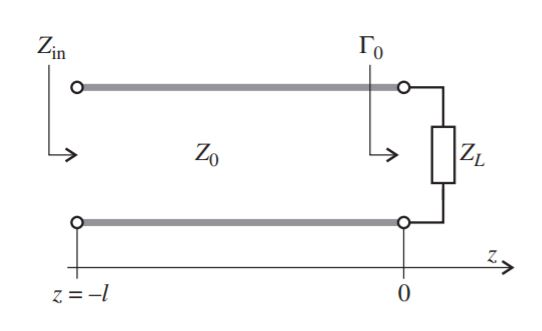
\includegraphics{./image/chapter2/2-23.jpg}

Figure 2-22, A whole circuit on the entire transmission line

    There's a incident wave coming from the source to the load. There's a
reflected wave coming from the load to the source. Let us define a ratio
of the reflected to the incident voltage wave called \textbf{reflection
coefficient \(\Gamma_0\)}.\[\Gamma_0 = \frac{V^-}{V^+}\]

    \begin{tcolorbox}[breakable, size=fbox, boxrule=1pt, pad at break*=1mm,colback=cellbackground, colframe=cellborder]
\prompt{In}{incolor}{ }{\boxspacing}
\begin{Verbatim}[commandchars=\\\{\}]

\end{Verbatim}
\end{tcolorbox}


    % Add a bibliography block to the postdoc
    
    
    
\end{document}
